\documentclass{article}
\usepackage[margin=1in]{geometry}
\usepackage{amsmath,amsthm,amssymb}
\usepackage{bbm,enumerate,mathtools}
\usepackage{tikz,pgfplots}
\usepackage{chessboard}
\usepackage[hidelinks]{hyperref}
\usepackage{multicol} % Problem 35
\usepackage{xstring} % Difficulty command
\usetikzlibrary{shapes.geometric}

\newenvironment{question}{\begin{trivlist}\item[\textbf{Question.}]}{\end{trivlist}}
\newenvironment{note}{\begin{trivlist}\item[\textbf{Note.}]}{\end{trivlist}}
\newenvironment{references}{\begin{trivlist}\item[\textbf{References.}]}{\end{trivlist}}
\newenvironment{related}{\begin{trivlist}\item[\textbf{Related.}]\end{trivlist}\begin{enumerate}}{\end{enumerate}}

\newcommand\score[1]{
\pgfmathsetmacro\pgfxa{#1+1}
\tikzstyle{scorestars}=[
  star,
  star points=5,
  star point ratio=2.25,
  draw,
  inner sep=3pt,
  anchor=outer point 5
]
  \begin{tikzpicture}[baseline]
    \draw[opacity=0] (0,-0.5) rectangle (0,0.2); % Workaround for whitespace at the bottom.
    \foreach \i in {1,...,4} {
      \pgfmathparse{(\i<=#1?"yellow":"gray")}
      \edef\starcolor{\pgfmathresult}
      \draw (\i*4.5ex,0) node[name=star\i,scorestars,fill=\starcolor]  {};
    }
  \end{tikzpicture}
}

\newcommand{\difficulty}[1]{%
  \IfEqCase{#1}{%
      {1}{
        
\begin{tikzpicture}[scale=0.7, baseline=0.9mm]%
          \definecolor{slopegreen}{rgb}{0.0, 0.5, 0.0}%
          \fill[slopegreen] (0.5,0.5) circle (0.5);%
        \end{tikzpicture}%
      }%
      {2}{
        
\begin{tikzpicture}[scale=0.7, baseline=0.9mm]%
          \definecolor{slopeblue}{rgb}{0.0, 0.44, 1.00}
          \fill[slopeblue] (0,0) rectangle (1,1);%
        \end{tikzpicture}%
      }%
      {3}{
\begin{tikzpicture}[scale=0.7, baseline=0.9mm]\fill (0,0.5)--(0.5, 0)--(1,0.5)--(0.5,1)--cycle; \end{tikzpicture}}%
      {4}{
\begin{tikzpicture}[scale=0.7, baseline=0.9mm]\fill (0.25,0)--(0,0.5)--(0.25,1)--(0.5,0.5)--cycle; \fill (0.75,0)--(0.5,0.5)--(0.75,1)--(1,0.5)--cycle;\end{tikzpicture}}%
      % you can add more cases here as desired
  }[\PackageError{difficulty}{Undefined difficulty level: #1}{}]%
}%
\newcommand{\rating}[2]{\difficulty{#1}\\\score{#2}\\}


\begin{document}
\rating{2}{3}
Consider ways to lay matchsticks (of unit length) on the $n \times m$ grid in
such a way as to form a maze.
\begin{figure}[ht!]
  \centering
  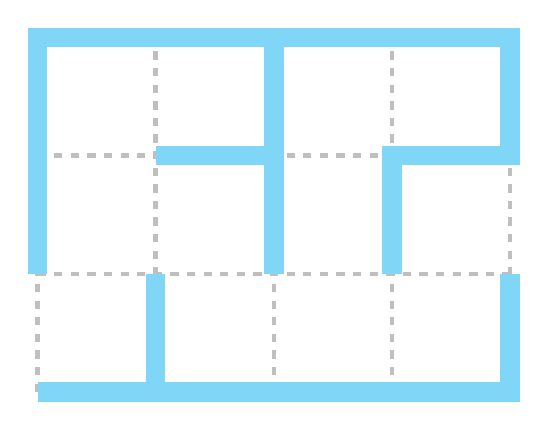
\begin{tikzpicture}[scale=1.5]
    \draw[ultra thick, gray!50, dashed] (0,0) grid (4,3);
    \draw[line width=0.25cm, cyan!50] (0,0)--(4,0)--(4,1);
    \draw[line width=0.25cm, cyan!50] (1,0)--(1,1);
    \draw[line width=0.25cm, cyan!50] (0,1)--(0,3)--(4,3)--(4,2)--(3,2)--(3,1);
    \draw[line width=0.25cm, cyan!50] (2,3)--(2,1);
    \draw[line width=0.25cm, cyan!50] (1,2)--(2,2);
  \end{tikzpicture}\hspace{0.5cm}
  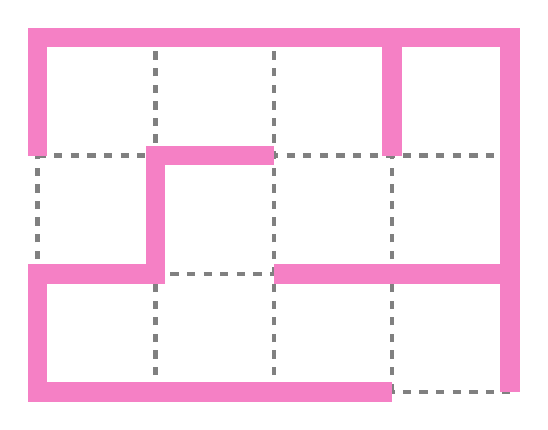
\begin{tikzpicture}[scale=1.5]
    \draw[ultra thick, gray, dashed] (0,0) grid (4,3);
    \draw[line width=0.25cm, magenta!50] (2,2)--(1,2)--(1,1)--(0,1)--(0,0)--(3,0);
    \draw[line width=0.25cm, magenta!50] (0,2)--(0,3)--(4,3)--(4,0);
    \draw[line width=0.25cm, magenta!50] (2,1)--(4,1);
    \draw[line width=0.25cm, magenta!50] (3,3)--(3,2);
    % \draw[line width=0.25cm, green!50] (4,0)--(4,1)--(2,1)--(2,0)--cycle;
  \end{tikzpicture}
  \caption{
    Two mazes on a $(5 \times 4)$-cell grid.
  }
\end{figure}
\begin{question}
  How many distinct mazes can be drawn on the grid?
\end{question}

\begin{related}
  \item What if every $1\times1$ cell must be reachable?
  \item What if there are no dead ends?
  \item What if there are to be identically $k$ dead ends?
  \item What if paths that loop are not allowed?
  \item What if the entrance and exit have prescribed positions?
  \item What if this is done on a hexagonal or triangular grid? On a torus?
  \item Is there a meaningful way to assign ``difficulty'' to a maze?
\end{related}
\begin{note}
  This appears to be the number of spanning trees on the $n \times m$ grid graph
  such that the start and end are leaves.
\end{note}
\begin{references}
  \item Problem 56.
  \item \url{https://oeis.org/A116469}
\end{references}
\end{document}
